\section{Dynamische Grundglieder (mit Gedächtnis)}

Der Ausgang des Systems ist vom aktuellen \textbf{und} von vergangenen Eingängen abhängig.
Vergangene Eingänge werden im System in einem Speicher, einem Zustand $x(t)$ abgelegt 
$$ y(t) = f( u(t), \, x(t) ) $$


\subsubsection{Prozesse mit / ohne Ausgleich}

\begin{tabular}{ll}
ohne Ausgleich: & Sprungantwort wächst grenzenlos an                    \\
mit Ausgleich:  & Sprungantwort strebt gegen endlichen Wert             \\
				& \textrightarrow\ \textbf{Gegenkopplung} am Ausgang 
\end{tabular}


\subsection{Totzeit-Glied}{30}

\vspace{-0.2cm}
$$ \boxed{ y(t) =  u(t - T_t) } $$

\begin{center}
    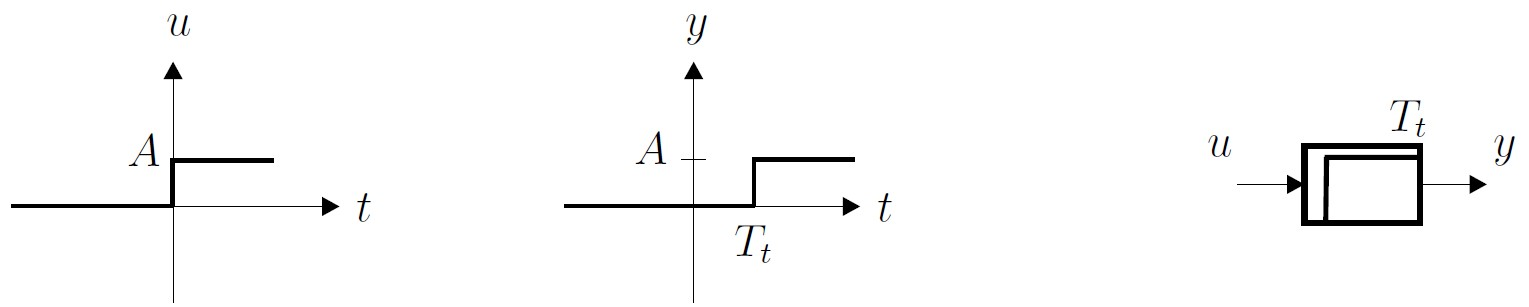
\includegraphics[width=0.9\columnwidth]{images/totzeit-glied.jpg}
\end{center}


\subsection{I-Glied (Integrierer)}{29}

\vspace{-0.3cm}
\begin{minipage}[c]{0.48\columnwidth}
    $$ \boxed{ \text{DGL:} \quad \dot{y}(t) = K \cdot u(t) }  $$
\end{minipage}
\hfill
\begin{minipage}[c]{0.48\columnwidth}
    $$ \boxed{ y = \int\limits_{- \infty}^t u(\tau) \, d \tau = K \int\limits_{- \infty}^t u(\tau) \, \diff \tau + y(0) } $$
\end{minipage}

\begin{center}
    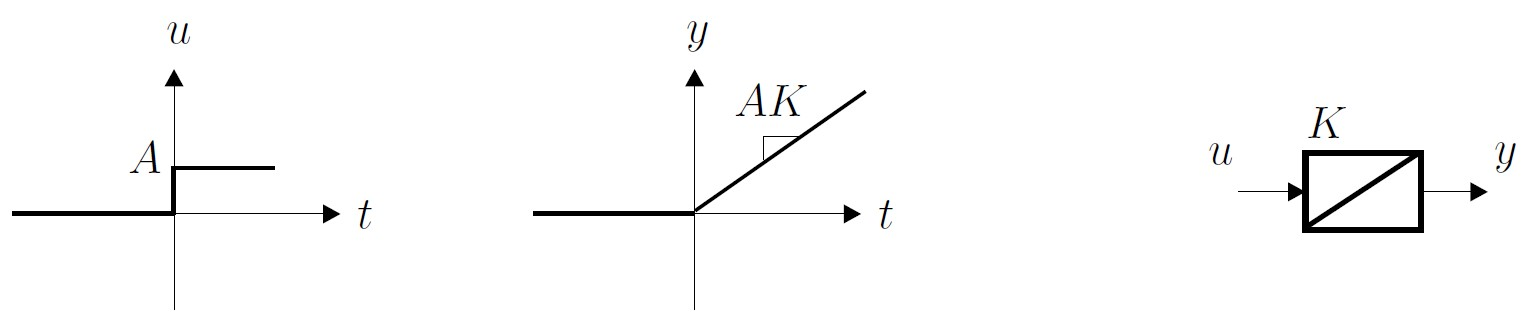
\includegraphics[width=0.9\columnwidth]{images/i-glied.jpg} 
\end{center}

\columnbreak


\subsection[PT1-Glied]{$\text{PT}_1$-Glied}{31-33}

Ein Energiespeicher \textrightarrow\ System schwingt \textbf{nicht}

\begin{minipage}[t]{0.48\columnwidth}
    $$ \boxed{ \text{DGL:} \quad  T \, \dot{y}(t) + y(t) = K \cdot u(t) }  $$
\end{minipage}
\hfill
\begin{minipage}[t]{0.48\columnwidth}
    $$ \boxed{ y(t) = K \, A + (y_0 - K \, A) \cdot e^{- \frac{t}{T}} } $$
\end{minipage}


\begin{minipage}{0.5\columnwidth}
    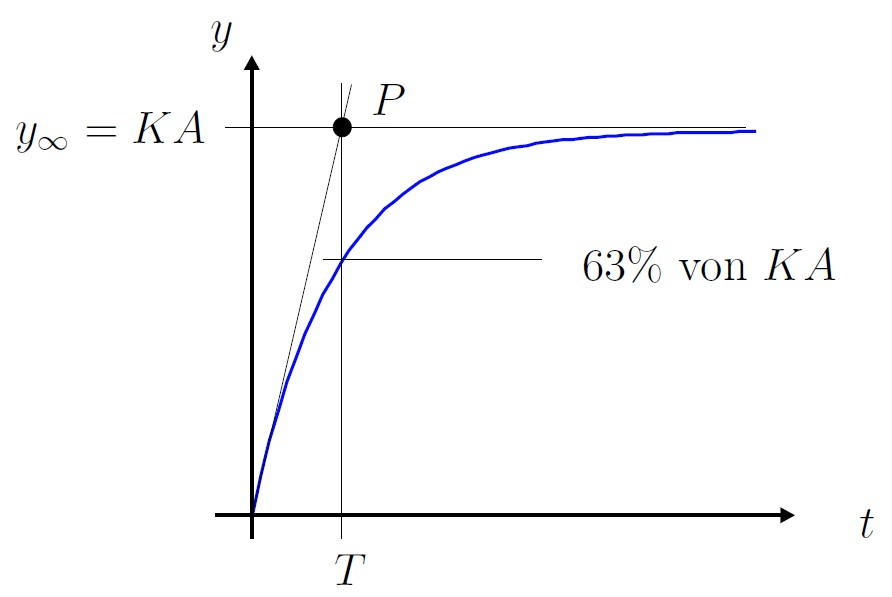
\includegraphics[width=\columnwidth]{images/pt1-glied_kennlinie.jpg}
\end{minipage}
\hfill
\begin{minipage}{0.4\columnwidth}
    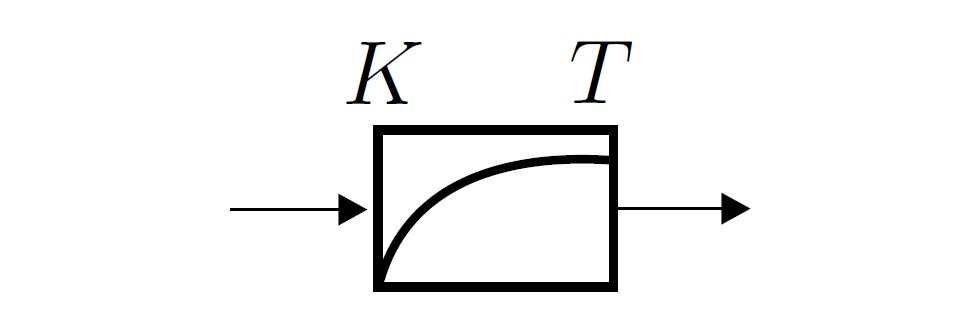
\includegraphics[width=0.8\columnwidth]{images/symbol_PT1-glied.jpg}
\end{minipage}


\subsubsection{Modellierung einer $\text{PT}_1$ Regelstrecke}

\begin{enumerate}
    \item Ausmessen der Sprungantwort $u(t) = A \cdot \varepsilon(t)$ \\
        \textrightarrow\ Die Sprungantwort entspricht dem Diagramm
    \item  Parameter $K$ berechnen: $K = \frac{y_\infty}{A}$
    \item Parameter $T$ bestimmen: Tangente am Anfang durch Punkt $P$ \\
        oder: Zeit bis $y(T) = 0.63 \cdot K \, A$ erreicht ist \textrightarrow\ $T$ ablesen
\end{enumerate}


\example{$\text{PT}_1$-Glied als Blockschaltbild}

\begin{minipage}[c]{0.48\columnwidth}
    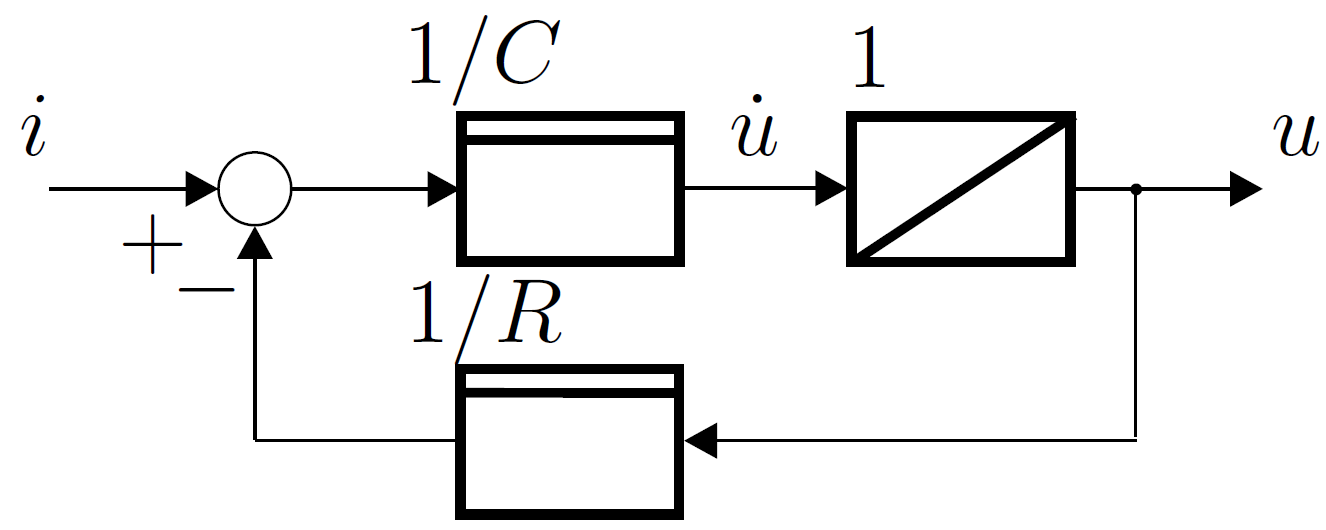
\includegraphics[width=\columnwidth]{images/pT1_blockschaltbild.png}
\end{minipage}
\hfill
\begin{minipage}[c]{0.48\columnwidth}
    $$ \boxed{ \text{Allg: } T \, \dot{y}(t) + y(t) = K \cdot u(t) } $$
    $$ \boxed{ \text{Bsp: } RC \, \dot{u}(t) + u(t) = R \cdot i(t) } $$
\end{minipage}


\subsection[PT2-Glied]{$\text{PT}_2$-Glied}{34}

Zwei Energiespeicher \textrightarrow\ \textbf{System kann schwingen}

\vspace{-0.2cm}

\begin{minipage}[c]{0.46\columnwidth}
    $$ \boxed{\text{DGL:} \quad T^2 \cdot  \ddot{y} + 2 \, \zeta \, T \cdot \dot{y} + y = K \cdot u } $$
\end{minipage}
\hfill
\begin{minipage}[c]{0.52\columnwidth}
    $$ \boxed{ y(t) = K \: A \Big[ 1 + e^{\sigma t} \big( - \cos(\omega t) + \frac{\sigma}{\omega} \sin(\omega t)  \big)  \Big] }  $$
\end{minipage}


\begin{minipage}{0.55\columnwidth}
    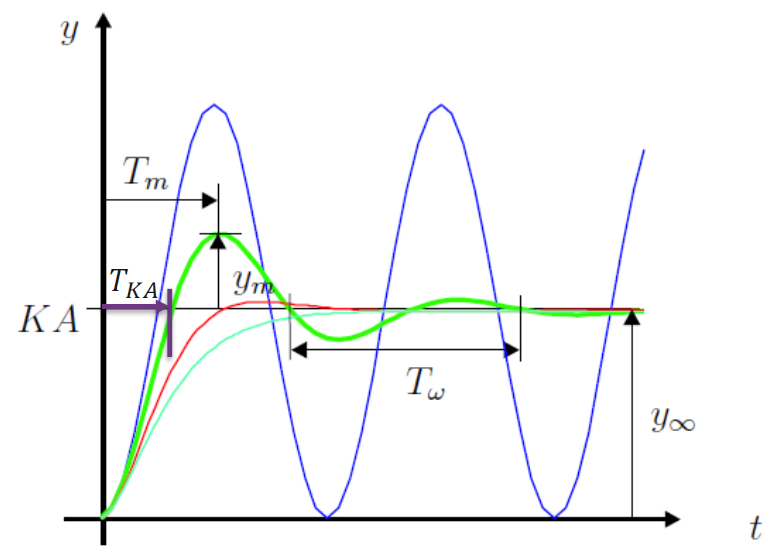
\includegraphics[width=\columnwidth]{images/pT2_sprungantwort.png}
\end{minipage}
\hfill
\begin{minipage}{0.38\columnwidth}
    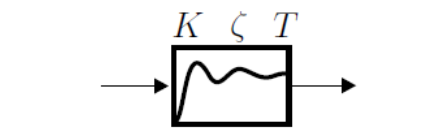
\includegraphics[width=0.75\columnwidth]{images/pT2_symbol.png}

    $$\omega = \omega_n \cdot \sqrt{1 - \zeta^2} $$
    $$ y_m = e^h \cdot y_{\infty} $$ 
\end{minipage}


\begin{center}
    \renewcommand{\arraystretch}{1.8}
    \begin{tabular}{c c c}
        $K = \frac{y_{\infty}}{A}$                                      & $h = \ln \big( \frac{y_m}{y_{\infty}} \big)$                                  & $\omega = \frac{2 \, \pi}{T_{\omega}} = \frac{\pi}{T_m}$  \\
        $\sigma = \frac{h \, \omega}{\pi} = - \omega_n \cdot \zeta$     & $\omega_n = \sqrt{\omega^2 + \sigma^2} = - \frac{\sigma}{\zeta}$              & $\zeta = - \frac{h}{\sqrt{h^2 + \pi^2}}$                  \\
        $T = \frac{1}{\omega_n}$                                        & $T_{KA} = T_M - \frac{1}{\omega} \arctan \big(  \frac{\omega}{\sigma} \big)$  & $y(T_{KA}) = K \: A$
    \end{tabular}
    \renewcommand{\arraystretch}{1}
\end{center}


\subsection{D-Glied (Idealer Differenzierer)}{37}

\vspace{-0.2cm}
$$ \boxed{  y(t) = K \cdot \frac{\diff \, u(t)}{\diff t} = K  \cdot \dot{u}(t) } $$

\begin{minipage}{0.25\columnwidth} 
    \begin{center}
        \textbf{ideal}\\
        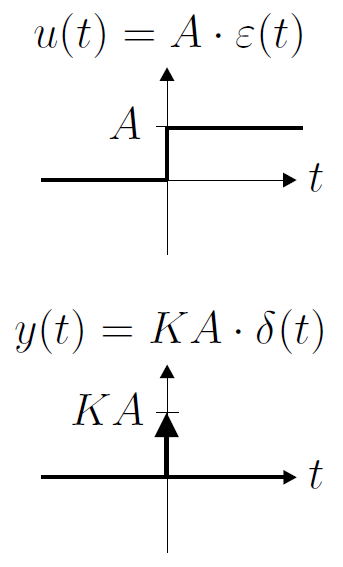
\includegraphics[width=0.9\columnwidth]{images/D-glied_ideal.png}
    \end{center}
\end{minipage}
\hfill
\begin{minipage}{0.25\columnwidth}
    \begin{center}
        \textbf{real}\\
        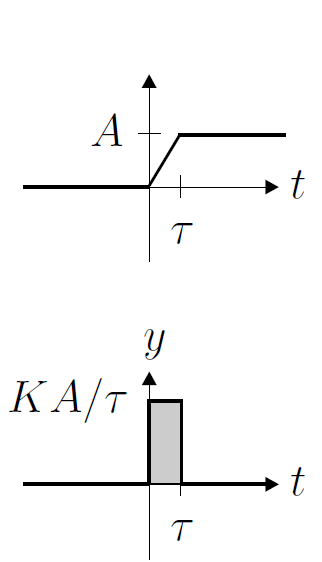
\includegraphics[width=0.9\columnwidth]{images/D-glied_real.png}
    \end{center}
\end{minipage}
\hfill
\begin{minipage}{0.25\columnwidth}
    \begin{center}
        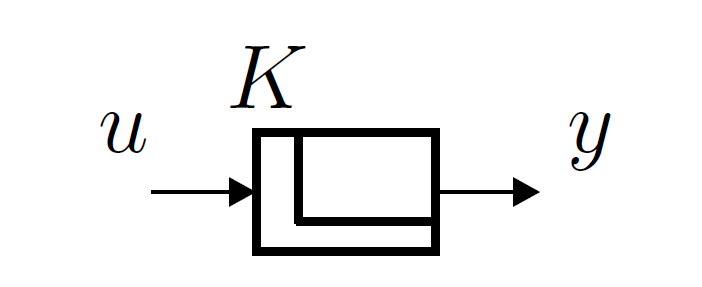
\includegraphics[width=0.9\columnwidth]{images/D-glied_symbol.png}
    \end{center}
\end{minipage}


\subsection[DT1-Glied (Realisierbarer Differenzierer)]{$\text{DT}_1$-Glied (Realisierbarer Differenzierer)}{38}

\begin{minipage}[c]{0.48\columnwidth}
    $$ \boxed{ w(t) = A \cdot (1 - e^{-\frac{t}{T}}) } $$
\end{minipage}
\hfill
\begin{minipage}[c]{0.48\columnwidth}
    $$ \boxed{ y(t) = \frac{K \cdot A}{T} \,  e^{-\frac{t}{T}} } $$
\end{minipage}

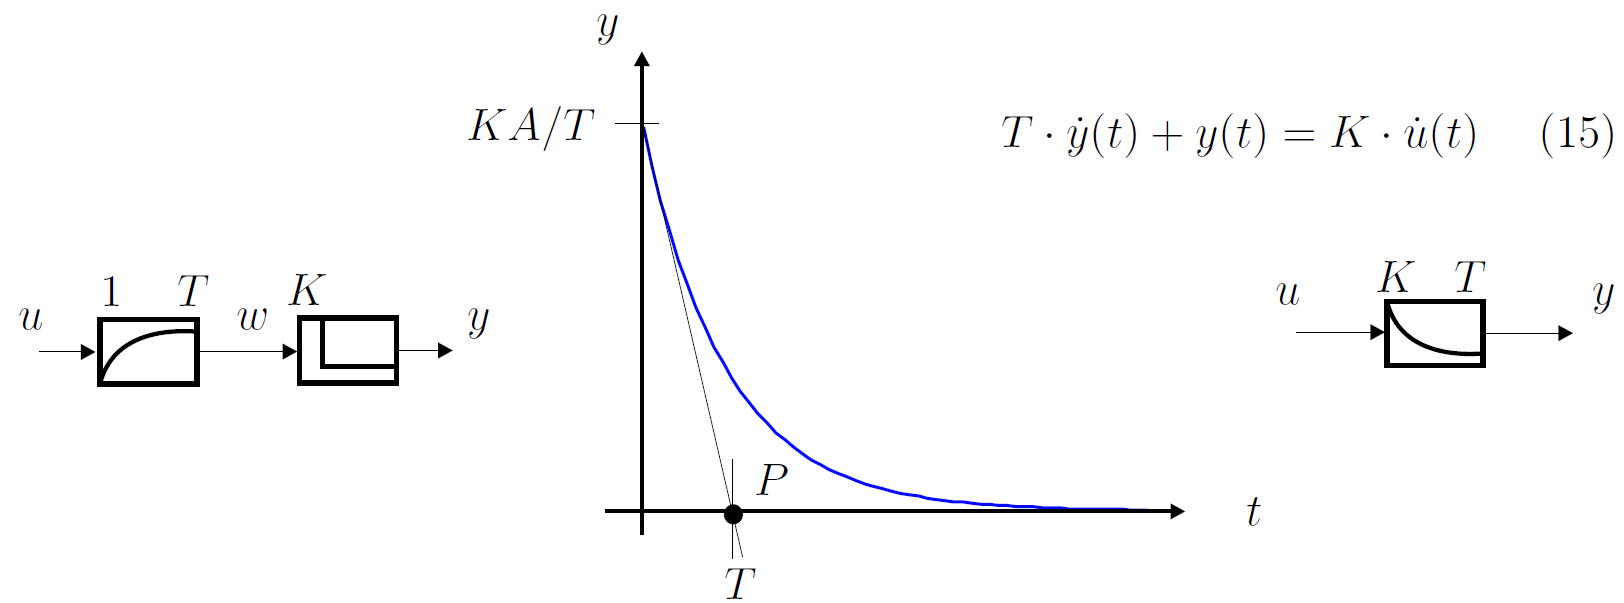
\includegraphics[width=\columnwidth]{images/DT1-glied.png}


\example{Mögliche Realisierungen von $\text{DT}_1$-Gliedern}

\begin{minipage}[t]{0.48\columnwidth}
    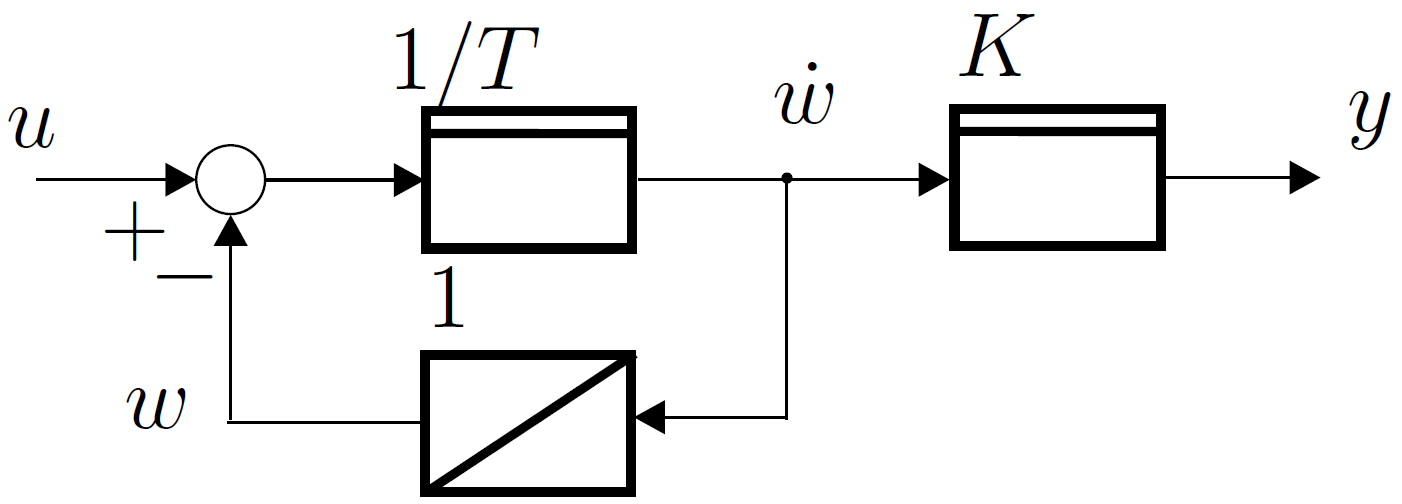
\includegraphics[width=\columnwidth, align=t]{images/pT1_blockschaltbild_2.png}
\end{minipage}
\hfill
\begin{minipage}[t]{0.48\columnwidth}
    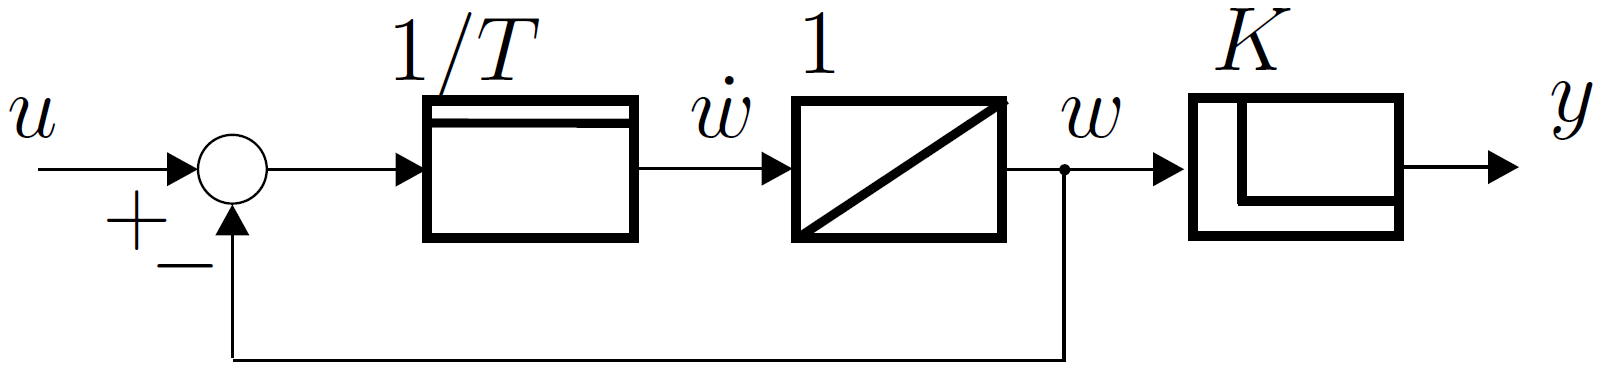
\includegraphics[width=\columnwidth, align=t]{images/DT1-glied_blockschaltbild.png}
\end{minipage}


\subsection{PID-Glied}{39}

\textbf{Zusammensetzen der Grundglieder: Parallelschaltung!} \\
Gilt auch für P, PI, PD, $\text{PDT}_1$ und $\text{PIDT}_1$ Glieder 
$$ \boxed{  y(t) = A \cdot \big[ K_P + K_I \cdot t + \frac{K_D}{T_C} e^{-\frac{t}{T_c}} \big]  }$$

\begin{minipage}{0.48\columnwidth}
    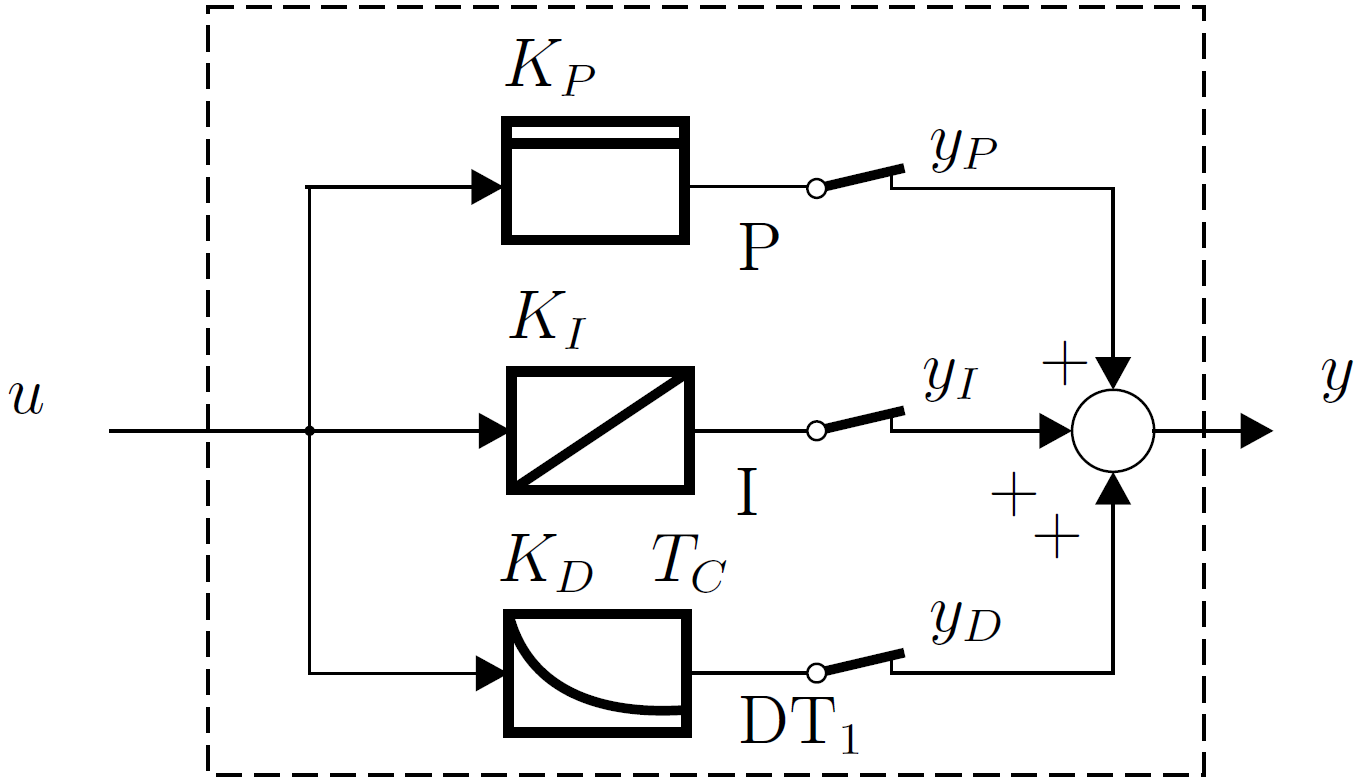
\includegraphics[width=0.9\columnwidth]{images/PID-glied.png}
\end{minipage}
\hfill
\begin{minipage}{0.5\columnwidth}
    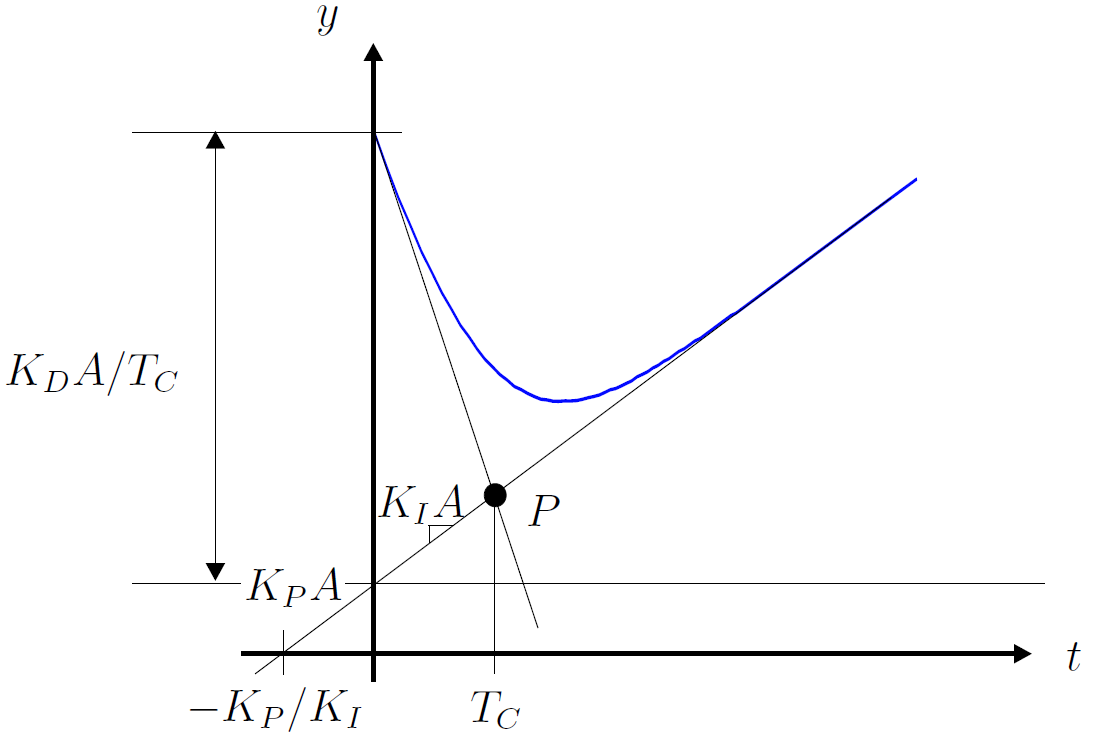
\includegraphics[width=\columnwidth]{images/PID_sprungantwort.png}
\end{minipage}


\subsection{Lead-Glied / Lag-Glied / Lead-Lag-Glied (S.40-41)}{40-41}

Lead-/ Lag-Glieder sind zwei Varianten von $\text{PDT}_1$-Gliedern. 

\vspace{0.2cm}
\begin{tabular}{ll}
    Lead:   & $K_P$ und $K_D$ haben \myul{gleiches} Vorzeichen          \\
    Lag:    & $K_P$ und $K_D$ haben \myul{unterschiedliches} Vorzeichen
\end{tabular}

\vspace{0.2cm}

Lead- und Lag-Glieder können auch als Parallelschaltungen eines P- und eines $\text{PT}_1$-Glieds aufgefasst werden. 

Das Lead-Lag-Glied  ist eine Serieschaltung aus Lead- und Lag-Glied.

\vspace{0.2cm}

\begin{minipage}{0.44\columnwidth}
    \begin{center}
        \textbf{Lead-Glied} \\
        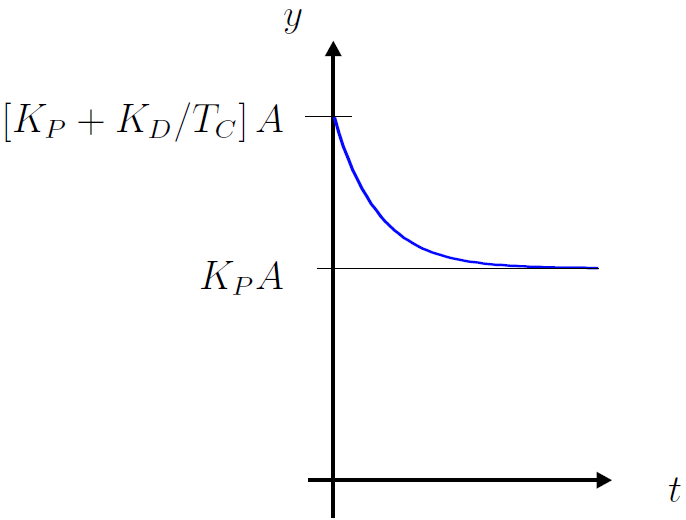
\includegraphics[width=\columnwidth]{images/lead-glied.png} 
    \end{center}
\end{minipage}
\hfill
\begin{minipage}{0.45\columnwidth}
    \begin{center}
        \textbf{Lag-Glied} \\
        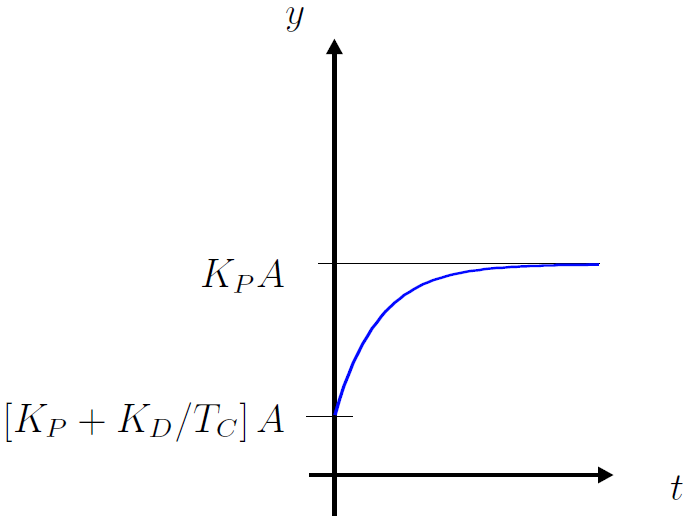
\includegraphics[width=\columnwidth]{images/lag-glied.png}
    \end{center}
\end{minipage}

